% Column-width ASAP7 die: cropped photo, labels on the blocks.
% Black pad so the layout is not flush-cut at the top and bottom.
\definecolor{tvink}{HTML}{111111}

\begin{tikzpicture}[
  tag/.style={
    draw=tvink,
    line width=0.5pt,
    rounded corners=1.2pt,
    fill=white,
    font=\sffamily\scriptsize\bfseries,
    align=center,
    inner xsep=3.0pt,
    inner ysep=1.6pt,
  },
]
\node[inner xsep=1.8mm, inner ysep=3.2mm, fill=black, outer sep=0] {
  \begin{tikzpicture}
    \node[inner sep=0, anchor=south west] (die) at (0,0)
      {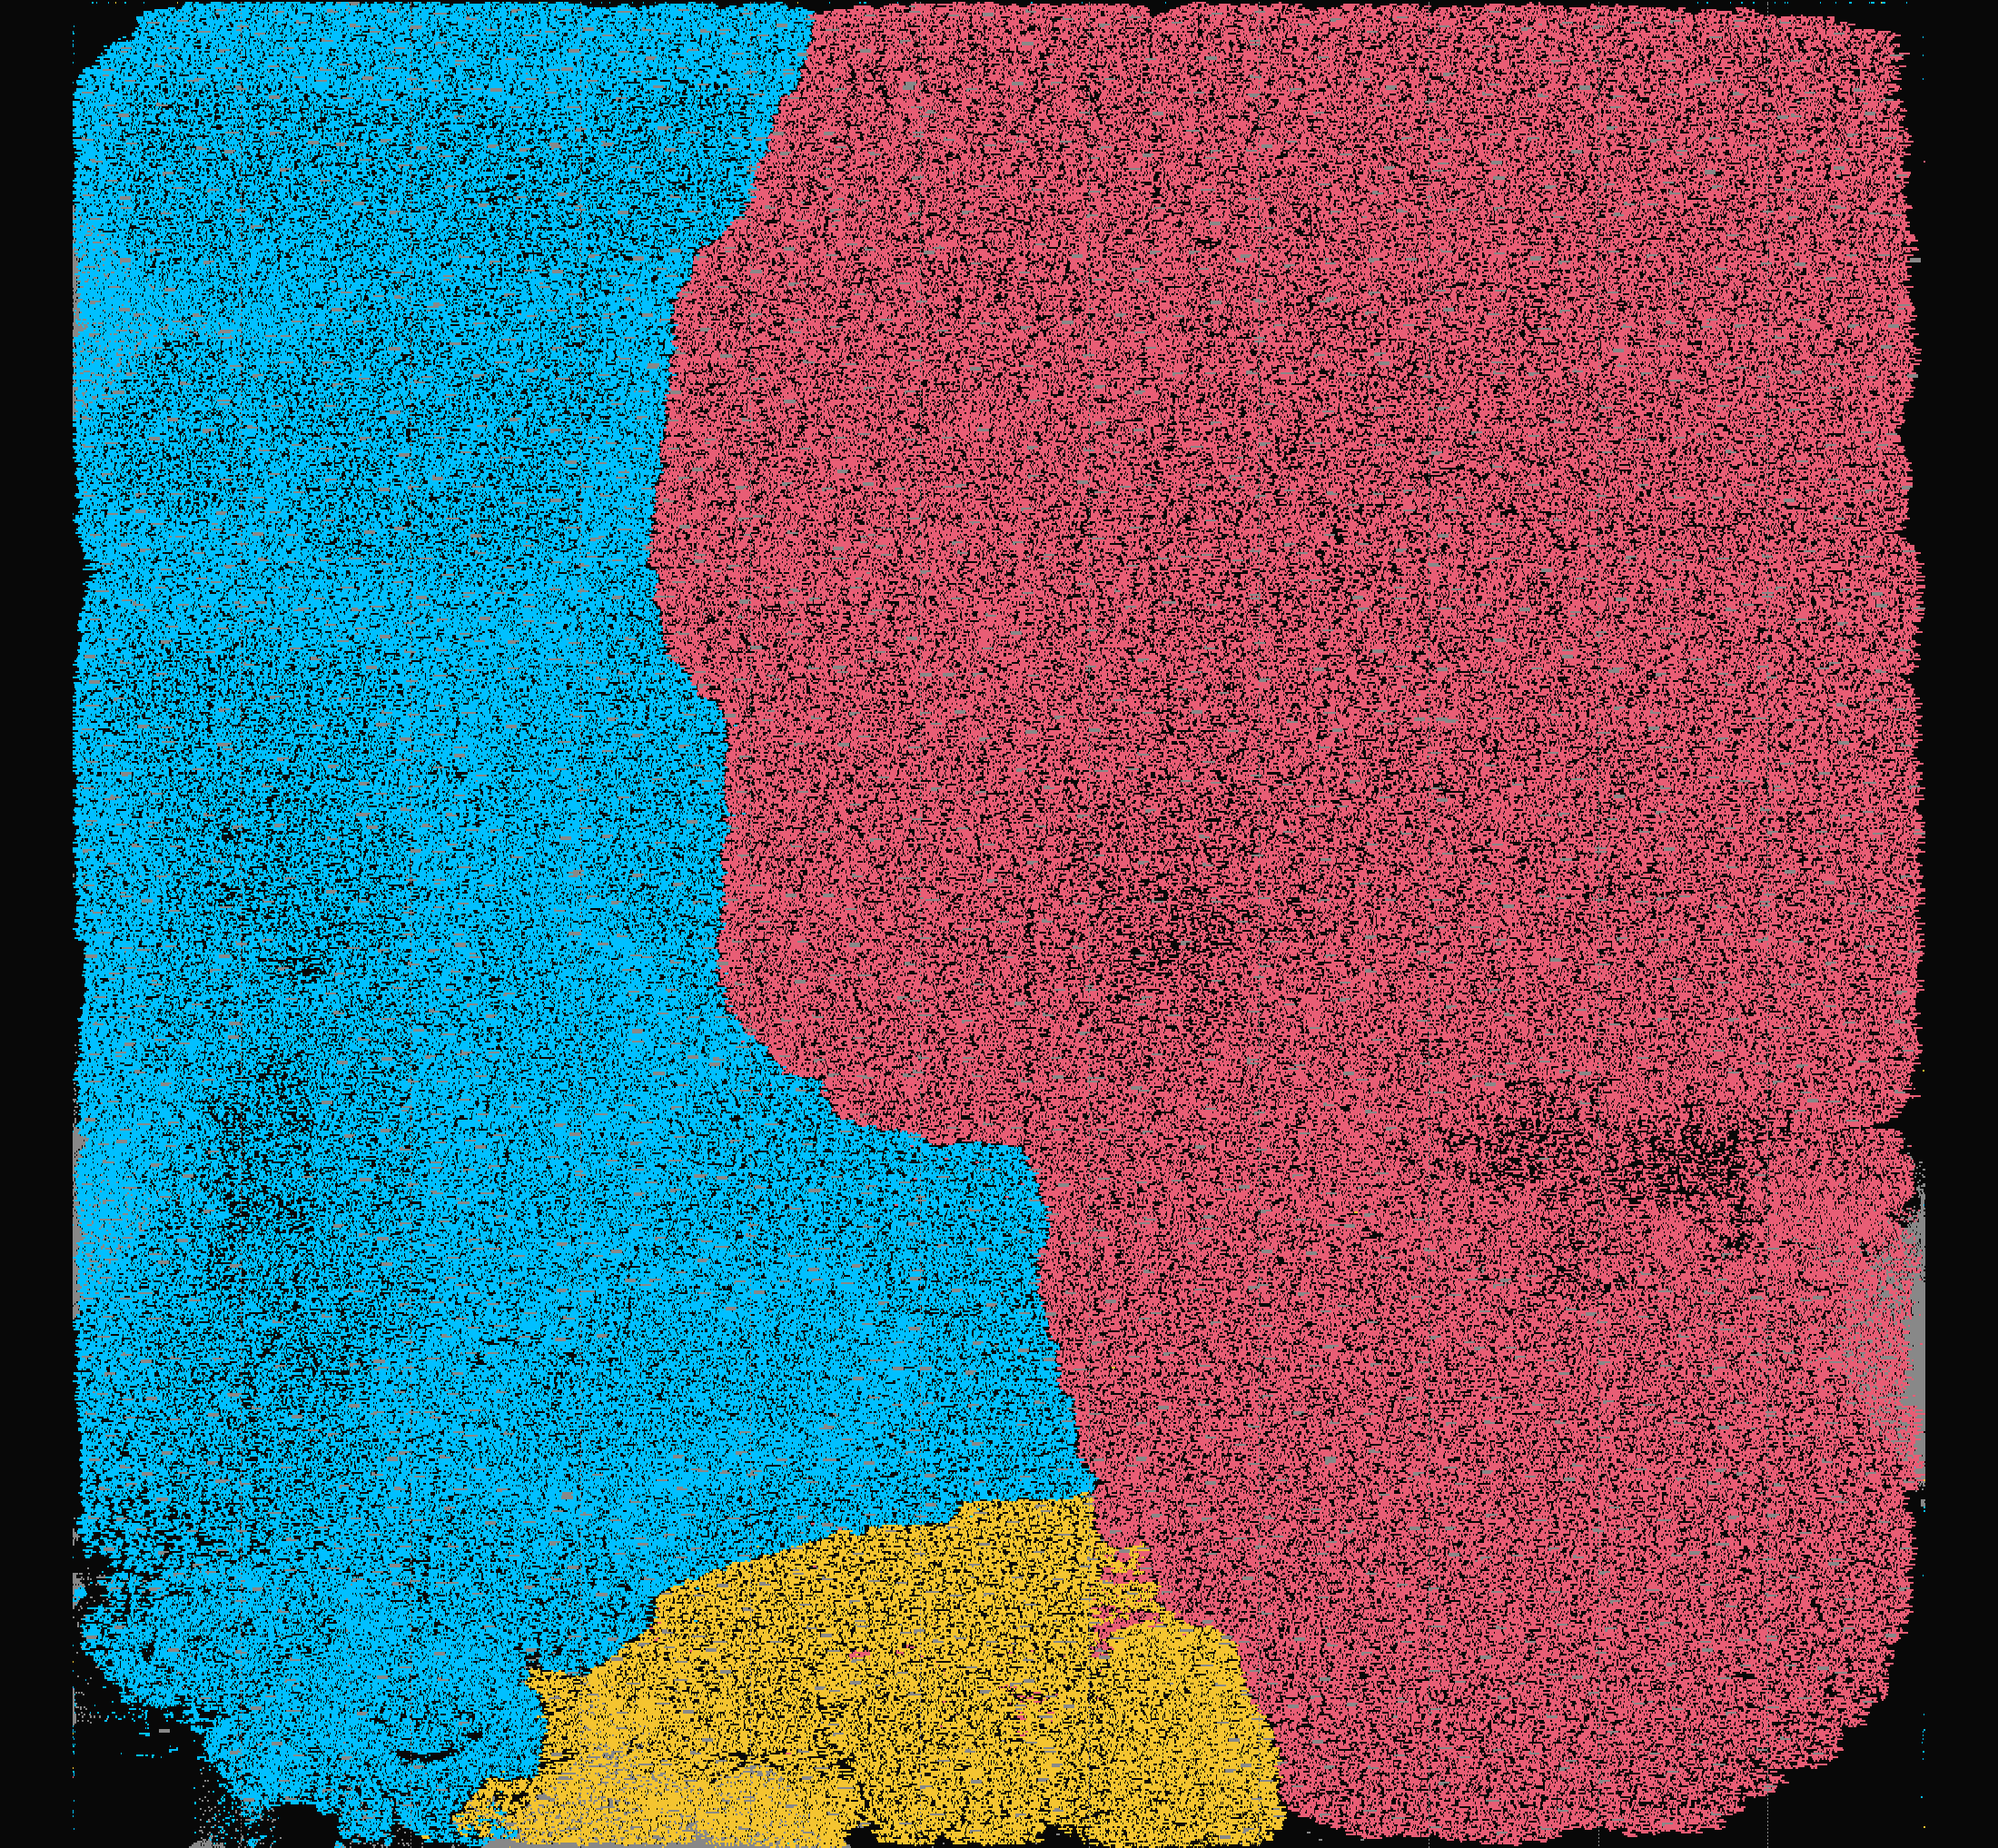
\includegraphics[width=\dimexpr\columnwidth-3.6mm\relax]{core_gemm_die}};
    \begin{scope}[x={(die.south east)}, y={(die.north west)}]
      \node[tag] at (0.22, 0.50) {GEMM};
      \node[tag] at (0.68, 0.56) {Vector};
      \node[tag] at (0.40, 0.11) {Core};
    \end{scope}
  \end{tikzpicture}
};
\end{tikzpicture}
